% Protokol: fotopřepínače (azobenzen), pch2b.
% Překlad: tectonic protokol.tex  nebo  xelatex protokol.tex (2x kvůli odkazům)
\documentclass[11pt,a4paper]{article}

% XeTeX potřebuje fontspec s OpenType fonty kvůli českým háčkům
\usepackage{fontspec}
\setmainfont{lmroman10-regular.otf}[BoldFont=lmroman10-bold.otf,
  ItalicFont=lmroman10-italic.otf, BoldItalicFont=lmroman10-bolditalic.otf]
\setsansfont{lmsans10-regular.otf}[BoldFont=lmsans10-bold.otf, ItalicFont=lmsans10-oblique.otf]
\setmonofont{lmmono10-regular.otf}[BoldFont=lmmonolt10-bold.otf, ItalicFont=lmmono10-italic.otf]
\usepackage{polyglossia}
\setmainlanguage{czech}
\usepackage{amsmath}
\usepackage{graphicx}
\usepackage{booktabs}
\usepackage{siunitx}
\usepackage{xcolor}
\usepackage[margin=2.5cm]{geometry}
\usepackage{caption}
\usepackage{float}
\usepackage[hidelinks]{hyperref}

% Česká sazba čísel: desetinná čárka, správné minus
\sisetup{output-decimal-marker={,}, per-mode=power, group-minimum-digits=5, separate-uncertainty=true,
  range-phrase={--}, list-pair-separator={ a~}, list-final-separator={ a~}, range-units=single, list-units=single}
\DeclareSIUnit\hartree{\ensuremath{E_\mathrm{h}}}
\newcommand{\kjm}{\si{\kilo\joule\per\mole}}
\newcommand{\cis}{\textit{cis}}
\newcommand{\trans}{\textit{trans}}
% značka pro místa, která musí autor doplnit nebo ověřit
\newcommand{\todo}[1]{\textcolor{red}{[K~revizi: #1]}}

\graphicspath{{../03-scan/}{../05-zindo/}{../06-orbitals/}}
\setlength{\parskip}{0.3em}
\setlength{\emergencystretch}{3em}
\widowpenalty=10000
\clubpenalty=10000

\title{Fotopřepínače}
\author{Aleš Toman}
\date{\today}

\begin{document}
\maketitle
\renewcommand{\refname}{Zdroje}

\section*{Zadání}
Azobenzen patří k~nejpoužívanějším fotopřepínačům. Úkolem bylo zvolit kvantově-chemickou metodu,
zoptimalizovat strukturu \trans\nobreakdash- a~\cis-azobenzenu, ověřit, že jde o~minima na hyperploše potenciální energie,
a~porovnat stabilitu obou izomerů. Dále provést optimalizovaný sken mezi oběma formami, spočítat izomerační
energii metodami PM6 a~\mbox{B3LYP/6-31G*} a~srovnat ji s~experimentem. Podél reakční koordináty měly být
metodou ZINDO spočteny energie základního a~dvou excitovaných stavů; nakonec zobrazit molekulové orbitaly
a~diskutovat charakter elektronových přechodů.

\section*{Úvod}
Fotopřepínače jsou molekuly, jejichž strukturu a~funkci lze řídit světlem. Azobenzen patří mezi
nejpoužívanější díky vratné izomeraci mezi formami \textit{E} a~\textit{Z}; změna geometrie může ovlivnit
vlastnosti molekuly i~její interakce s~okolím~\cite{Jiang2026,Gao2022}. V~současných technologiích se
azobenzenové přepínače zkoumají pro fotofarmakologickou regulaci biologických cílů, fotoresponzivní
supramolekulární systémy, aktuátory a~optické či energetické materiály~\cite{Jiang2026,Gao2022}.

Klasické azobenzeny se často aktivují UV světlem, jehož omezený průnik a~možnost poškození tkání či materiálů
motivují vývoj přepínačů reagujících na viditelné světlo~\cite{Gao2022,Li2025}. Jejich vlastnosti lze
upravovat chemickou substitucí a~změnou struktury; při návrhu je třeba zohlednit nejen absorpční vlnovou
délku, ale také účinnost přepnutí a~stabilitu izomerů~\cite{Li2025,Ryazantsev2021}. V~této úloze budou
\trans\nobreakdash- a~\cis-azobenzen porovnány pomocí kvantově-chemických výpočtů a~jejich izomerační dráha
bude analyzována z~hlediska energetiky a~elektronových stavů.

Přechod mezi izomery se obvykle popisuje dvěma cestami: rotací (torzí) kolem vazby N=N, kterou
vystihuje dihedrální úhel CNNC, a~inverzí na jednom z~dusíků, kterou vystihuje úhel CNN~\cite{Cembran2004}.
Proto jsme skenovali obě souřadnice. U~torze kolem \SI{90}{\degree} je vazba $\pi$ přerušená a~molekula má
diradikálový charakter, který uzavřenoslupkový (restricted, RKS) výpočet nepopíše; zde jsme použili
neomezený (UKS) výpočet s~narušenou symetrií (broken symmetry, BS), triplet a~Yamaguchiho spinovou
projekci~\cite{Yamaguchi1988}.

\section*{Metody}

\paragraph{Volba metody.}
Pro optimalizace, frekvence a~skeny jsme zvolili funkcionál $\omega$B97X-D3~\cite{Lin2013} s~bází
def2-TZVP~\cite{Weigend2005}. Jde o~hybridní funkcionál s~oddělením krátkého a~dlouhého dosahu
(range-separated), který obsahuje empirickou disperzní korekci D3. Disperzi jsme chtěli mít v~metodě
zahrnutou, protože v~\cis-izomeru jsou oba fenyly blízko sebe. Báze triple-zeta s~polarizačními funkcemi
je pro molekulu o~24 atomech ještě dostupná (optimalizace jednoho izomeru trvala asi \SI{15}{\minute}
na 8 jádrech). \todo{doplnit vlastní zdůvodnění, případně s~odkazem na benchmark}

\paragraph{Výpočty.}
Všechny výpočty DFT a~ZINDO/S proběhly v~programu ORCA~6.1.1~\cite{Neese2025} s~integrační mřížkou
DefGrid3 a~konvergenčním kritériem SCF \SI{e-9}{\hartree} (VeryTightSCF); geometrie byly optimalizovány
s~kritérii TightOpt. Minima jsme ověřili analytickým výpočtem frekvencí; termochemické veličiny jsou
v~harmonické aproximaci při \SI{298.15}{\kelvin} a~\SI{1}{atm}. Energie převádíme vztahem
\SI{1}{\hartree} = \SI{2625.4996}{\kilo\joule\per\mole}.

Relaxované skeny začínaly z~optimalizovaných minim s~krokem \SI{5}{\degree}: dihedrální úhel CNNC od
\SIrange{180}{0}{\degree} a~úhel CNN od \trans\ i~od \cis\ strany až k~lineárnímu uspořádání
(\SI{180}{\degree}). Ostatní souřadnice se v~každém bodě optimalizovaly. Protože skeny přeskakovaly mezi
různými konformacemi fenylů (viz Výsledky), přepočítali jsme kritické úseky z~druhé větve a~jako
reakční profil bereme dolní obálku, tj.\ v~každém bodě nejnižší energii ze všech větví. Tranzitní stav
inverze jsme optimalizovali metodou OptTS z~bodu CNN = \SI{180}{\degree} s~výpočtem Hessiánu.

U~torze \SI{90}{\degree} jsme otestovali stabilitu uzavřenoslupkového řešení a~spočítali singlet
s~narušenou symetrií a~triplet (UKS), oba s~CNNC fixovaným na \SI{90}{\degree}. Energii čistého singletu
$E_\mathrm{S}$ jsme odhadli Yamaguchiho projekcí~\cite{Yamaguchi1988}
\begin{equation}
  E_\mathrm{S} = E_\mathrm{BS} + \frac{\langle S^2\rangle_\mathrm{BS}}
    {\langle S^2\rangle_\mathrm{T} - \langle S^2\rangle_\mathrm{BS}}\,\bigl(E_\mathrm{BS} - E_\mathrm{T}\bigr),
  \label{eq:yamaguchi}
\end{equation}
kde $E_\mathrm{BS}$ a~$E_\mathrm{T}$ jsou energie řešení s~narušenou symetrií a~tripletu na stejné
geometrii a~$\langle S^2\rangle$ jsou příslušné střední hodnoty kvadrátu celkového spinu.

Izomerační energie metodou \mbox{B3LYP/6-31G*}~\cite{Becke1993,Lee1988} jsme počítali v~ORCA
(optimalizace a~frekvence, start z~geometrií $\omega$B97X-D3). Metodou PM6~\cite{Stewart2007} jsme
počítali v~programu MOPAC~23.2.5~\cite{MOPAC}; jejím výsledkem je přímo slučovací entalpie při
\SI{298}{\kelvin}, takže izomerační entalpie je rozdíl slučovacích entalpií obou izomerů.

Excitované stavy podél reakčních cest jsme počítali semiempirickou metodou ZINDO/S~\cite{Ridley1973}
s~konfigurační interakcí jednonásobných excitací (CIS, dva singletní kořeny) na geometriích dolní
obálky obou skenů. Energie stavů zobrazujeme jako $E(S_n) = E(S_0) + \Delta E_n$, kde $\Delta E_n$ je
vertikální excitační energie $n$-tého stavu. Na geometriích minim jsme vypsali koeficienty orbitalů
a~charakter orbitalů (podíl na dusících, podíl $p$-funkcí kolmých na rovinu CNNC) jsme určili skriptem
\texttt{mo\_character.py}. Vstupy, výstupy a~skripty jsou v~repozitáři
\url{https://github.com/alestoman5/photoswitch}; postup každého kroku popisují soubory \texttt{NOTES.md}.
\todo{ověřit, že je repozitář veřejný, jinak odkaz vynechat}

\section*{Výsledky a~diskuse}

\subsection*{Struktura a~stabilita izomerů}
Optimalizovaný \trans-azobenzen je planární, v~\cis-izomeru jsou fenyly vytočené z~roviny CNNC
(tabulka~\ref{tab:geom}). Ani jeden izomer nemá imaginární frekvenci; nejnižší frekvence je
\SI{12.0}{\per\centi\metre} pro \trans\ a~\SI{40.6}{\per\centi\metre} pro \cis. Obě struktury tedy leží
v~minimu na hyperploše potenciální energie. \trans-izomer je stabilnější: \cis\ leží o~\SI{50.9}{\kilo\joule\per\mole}
výše v~elektronové energii a~o~\SI{52.4}{\kilo\joule\per\mole} výše v~Gibbsově energii. Korekce na nulové
kmity a~termální příspěvky mění rozdíl jen o~jednotky \kjm.

\begin{table}[H]
\centering\small
\caption{Geometrie a~relativní energie \cis\ vůči \trans, $\omega$B97X-D3/def2-TZVP, \SI{298.15}{\kelvin}.
  $d$(N=N) délka vazby N=N, $\Delta E$ rozdíl elektronových energií, ZPE energie nulových kmitů,
  $\Delta H$ rozdíl entalpií, $\Delta G$ rozdíl Gibbsových energií.}
\label{tab:geom}
\begin{tabular}{lSSS@{\hspace{2em}}SSSS}
\toprule
 & {CNNC} & {CNN} & {$d$(N=N)} & {$\Delta E$} & {$\Delta E$+ZPE} & {$\Delta H$} & {$\Delta G$} \\
 & {/ \si{\degree}} & {/ \si{\degree}} & {/ \si{\angstrom}} & {/ \kjm} & {/ \kjm} & {/ \kjm} & {/ \kjm} \\
\midrule
\trans & 180.0 & 115.1 & 1.235 & 0 & 0 & 0 & 0 \\
\cis   & 5.8   & 122.6 & 1.231 & 50.9 & 50.4 & 50.0 & 52.4 \\
\bottomrule
\end{tabular}
\end{table}

\subsection*{Izomerační energie a~srovnání s~experimentem}
Tabulka~\ref{tab:iso} srovnává izomerační energie třemi metodami s~experimentem. $\omega$B97X-D3
dává izomerační entalpii \SI{50.0}{\kilo\joule\per\mole}, o~\SI{2.6}{\kilo\joule\per\mole} více než
hodnota pro plynnou fázi; rozdíl leží v~mezích její nejistoty. \mbox{B3LYP/6-31G*} stabilitu \trans-izomeru
nadhodnocuje asi o~\SI{14}{\kilo\joule\per\mole}. PM6 dává opačné znaménko, \cis\ podle ní vychází
o~\SI{16.5}{\kilo\joule\per\mole} stabilnější. Oba izomery jsme v~PM6 počítali se stejným nastavením
a~oba mají všechny frekvence kladné, chybné znaménko tedy jde na vrub metody, ne nastavení výpočtu.
PM6 navíc dává delší vazbu N=N u~\trans\ (\SI{1.254}{\angstrom}) a~větší úhel CNN u~\cis\
(\SI{128.6}{\degree}) než $\omega$B97X-D3.

\begin{table}[H]
\centering\small
\caption{Izomerační energie (\cis${}-{}$\trans) v~\kjm, plynná fáze, \SI{298.15}{\kelvin}. U~PM6 je
  $\Delta H$ rozdíl slučovacích entalpií; ostatní veličiny PM6 nedává. Čísla v~závorce jsou nejistoty
  posledních číslic.}
\label{tab:iso}
\begin{tabular}{lSSSS}
\toprule
metoda & {$\Delta E$} & {$\Delta E$+ZPE} & {$\Delta H$} & {$\Delta G$} \\
\midrule
$\omega$B97X-D3/def2-TZVP & 50.9 & 50.4 & 50.0 & 52.4 \\
\mbox{B3LYP/6-31G*}       & 63.5 & 61.9 & 61.9 & 62.8 \\
PM6                       & {--} & {--} & -16.5 & {--} \\
\midrule
exp., plynná fáze~\cite{Zhu2018,Cammenga2009} & {--} & {--} & 47.4(32) & {--} \\
exp., kapalina (DSC)~\cite{Zhu2018}           & {--} & {--} & 47.0(13) & {--} \\
\bottomrule
\end{tabular}
\end{table}
\todo{ověřit hodnoty 47,4(32) a~47,0(13) a~jejich přiřazení ke zdrojům v~plném textu \cite{Zhu2018,Cammenga2009}}

\subsection*{Izomerační cesty}
Obrázek~\ref{fig:scan} ukazuje relaxované skeny obou souřadnic. Sken torze z~\trans-izomeru mezi
\SIlist{80;75}{\degree} přeskočil na jinou větev: oba fenyly se přetočily a~energie klesla
o~\SI{96}{\kilo\joule\per\mole}, zatímco geometrie skupiny CN=NC zůstala spojitá. Přepočet z~druhé větve
dává u~\SIrange{80}{90}{\degree} nižší energie. Obdobně u~inverze se mezi \SIlist{155;160}{\degree} invertující
fenyl vytočil z~roviny kolmo (pokles o~\SI{2.5}{\kilo\joule\per\mole}). Maximum dolní obálky torze
(\SI{222.6}{\kilo\joule\per\mole} při \SI{90}{\degree}) leží v~průsečíku dvou větví, není to tedy
stacionární bod, ale hrot obálky.

\begin{figure}[H]
\centering
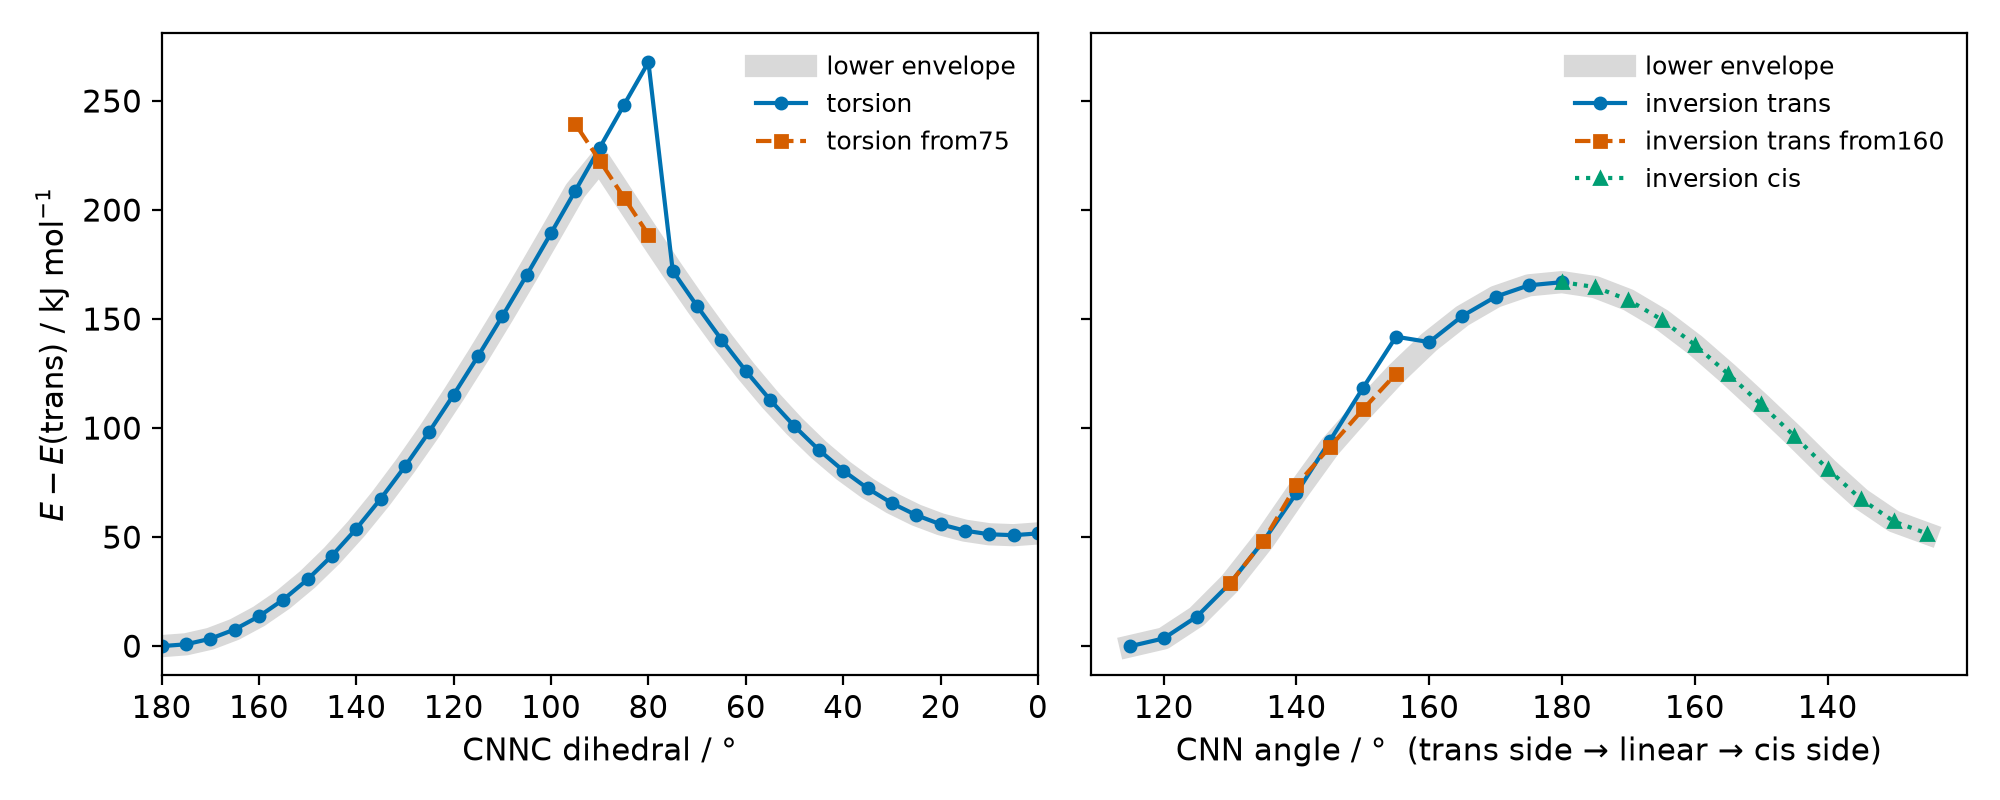
\includegraphics[width=\linewidth]{scan_envelope.png}
\caption{Relaxované skeny, $\omega$B97X-D3/def2-TZVP, energie vztažená k~\trans-izomeru. Vlevo torze CNNC,
  vpravo inverze CNN (\trans\ strana $\to$ lineární CNN $\to$ \cis\ strana, osa pokračuje jako
  $\SI{360}{\degree}-\mathrm{CNN}$). Šedě dolní obálka ze všech větví skenu.}
\label{fig:scan}
\end{figure}

Tranzitní stav inverze má jedinou imaginární frekvenci \SI{-421}{\per\centi\metre}; posun podél ní vede
na jednu stranu k~\trans\ a~na druhou k~\cis\ formě. V~tranzitním stavu je úhel CNN na invertujícím dusíku
\SI{179.4}{\degree} a~vazba N=N se zkrátí na \SI{1.209}{\angstrom}. Leží \SI{166.9}{\kilo\joule\per\mole}
nad \trans\ a~\SI{116.0}{\kilo\joule\per\mole} nad \cis\ (tabulka~\ref{tab:bar}).

Uzavřenoslupkové řešení u~torze \SI{90}{\degree} je nestabilní: matice stability má záporné vlastní číslo
(\SI{-0.0570}{\hartree}) a~výpočet přejde do UKS řešení s~$\langle S^2\rangle \approx 1$, tedy směsi
singletu a~tripletu. Energie \SI{222.6}{\kilo\joule\per\mole} ze skenu je proto výrazně nadhodnocená.
Po optimalizaci (CNNC fixován) leží singlet s~narušenou symetrií \SI{139.6}{\kilo\joule\per\mole} nad \trans,
projektovaný singlet podle rovnice~\eqref{eq:yamaguchi} \SI{155.5}{\kilo\joule\per\mole} a~triplet
\SI{124.2}{\kilo\joule\per\mole}. Triplet leží pod singletem, projekce proto energii singletu zvyšuje.
Projektovaná energie je spočtena na geometrii optimalizované pro BS řešení, ne ve vlastním minimu.

\begin{table}[H]
\centering\small
\caption{Energie bodů na izomeračních cestách, $\omega$B97X-D3/def2-TZVP, elektronová energie bez ZPE.
  $\langle S^2\rangle$ střední hodnota kvadrátu spinu. U~torze \SI{90}{\degree} je CNNC fixován.}
\label{tab:bar}
\begin{tabular}{lSSS}
\toprule
 & {$\langle S^2\rangle$} & {$\Delta E$ vůči \trans\ / \kjm} & {$\Delta E$ vůči \cis\ / \kjm} \\
\midrule
inverze, tranzitní stav                       & 0    & 166.9 & 116.0 \\
torze \SI{90}{\degree}, RKS (sken)             & 0    & 222.6 & 171.7 \\
torze \SI{90}{\degree}, BS singlet, opt.       & 1.10 & 139.6 & 88.6 \\
torze \SI{90}{\degree}, singlet (projekce)     & 0    & 155.5 & 104.6 \\
torze \SI{90}{\degree}, triplet, opt.          & 2.08 & 124.2 & 73.3 \\
\bottomrule
\end{tabular}
\end{table}

Pro termální zpětnou izomeraci \cis${}\to{}$\trans\ přes inverzi dostáváme
$\Delta H^\ddagger = \SI{110.8}{\kilo\joule\per\mole}$, $\Delta G^\ddagger = \SI{108.4}{\kilo\joule\per\mole}$
a~aktivační energii $E_\mathrm{a} = \Delta H^\ddagger + RT = \SI{113.3}{\kilo\joule\per\mole}$
(unimolekulární reakce v~plynné fázi, $R$ plynová konstanta, $T = \SI{298.15}{\kelvin}$). Měření
v~plynné fázi při \SIrange{181}{322}{\celsius} dalo \SI{118}{\kilo\joule\per\mole} a~autoři ho
interpretovali inverzním mechanismem~\cite{Andersson1982}. Na torzní cestě však leží triplet
i~projektovaný singlet níže než tranzitní stav inverze. Podle výpočtů Cembrana a~spol.\ může termální
izomerace probíhat torzí s~přechodem $S_0 \to T_1 \to S_0$ v~oblasti, kde se křivky $S_0$ a~$T_1$
kříží~\cite{Cembran2004}. Náš výpočet tento mechanismus nevylučuje, ale rychlost neadiabatického
přechodu jsme nepočítali, takže o~mechanismu nerozhoduje.

\subsection*{Excitované stavy podél reakční koordináty}
Obrázek~\ref{fig:zindo} ukazuje stavy $S_0$, $S_1$ a~$S_2$ ze ZINDO/S podél obou cest. Energie
základního stavu ze ZINDO/S nemá fyzikální smysl: \cis\ vychází \SI{157}{\electronvolt} nad \trans,
podél inverze má $S_0$ minimum u~CNN \SI{135}{\degree} (\SI{-12}{\electronvolt}) a~u~torze
\SI{90}{\degree} skáče o~desítky eV. ZINDO/S je parametrizována pro spektroskopii~\cite{Ridley1973}
a~celková energie se podél cesty mění hlavně s~jaderným odpuzováním. Interpretovat proto lze jen
excitační energie $\Delta E_n$ (dolní panely).

\begin{figure}[H]
\centering
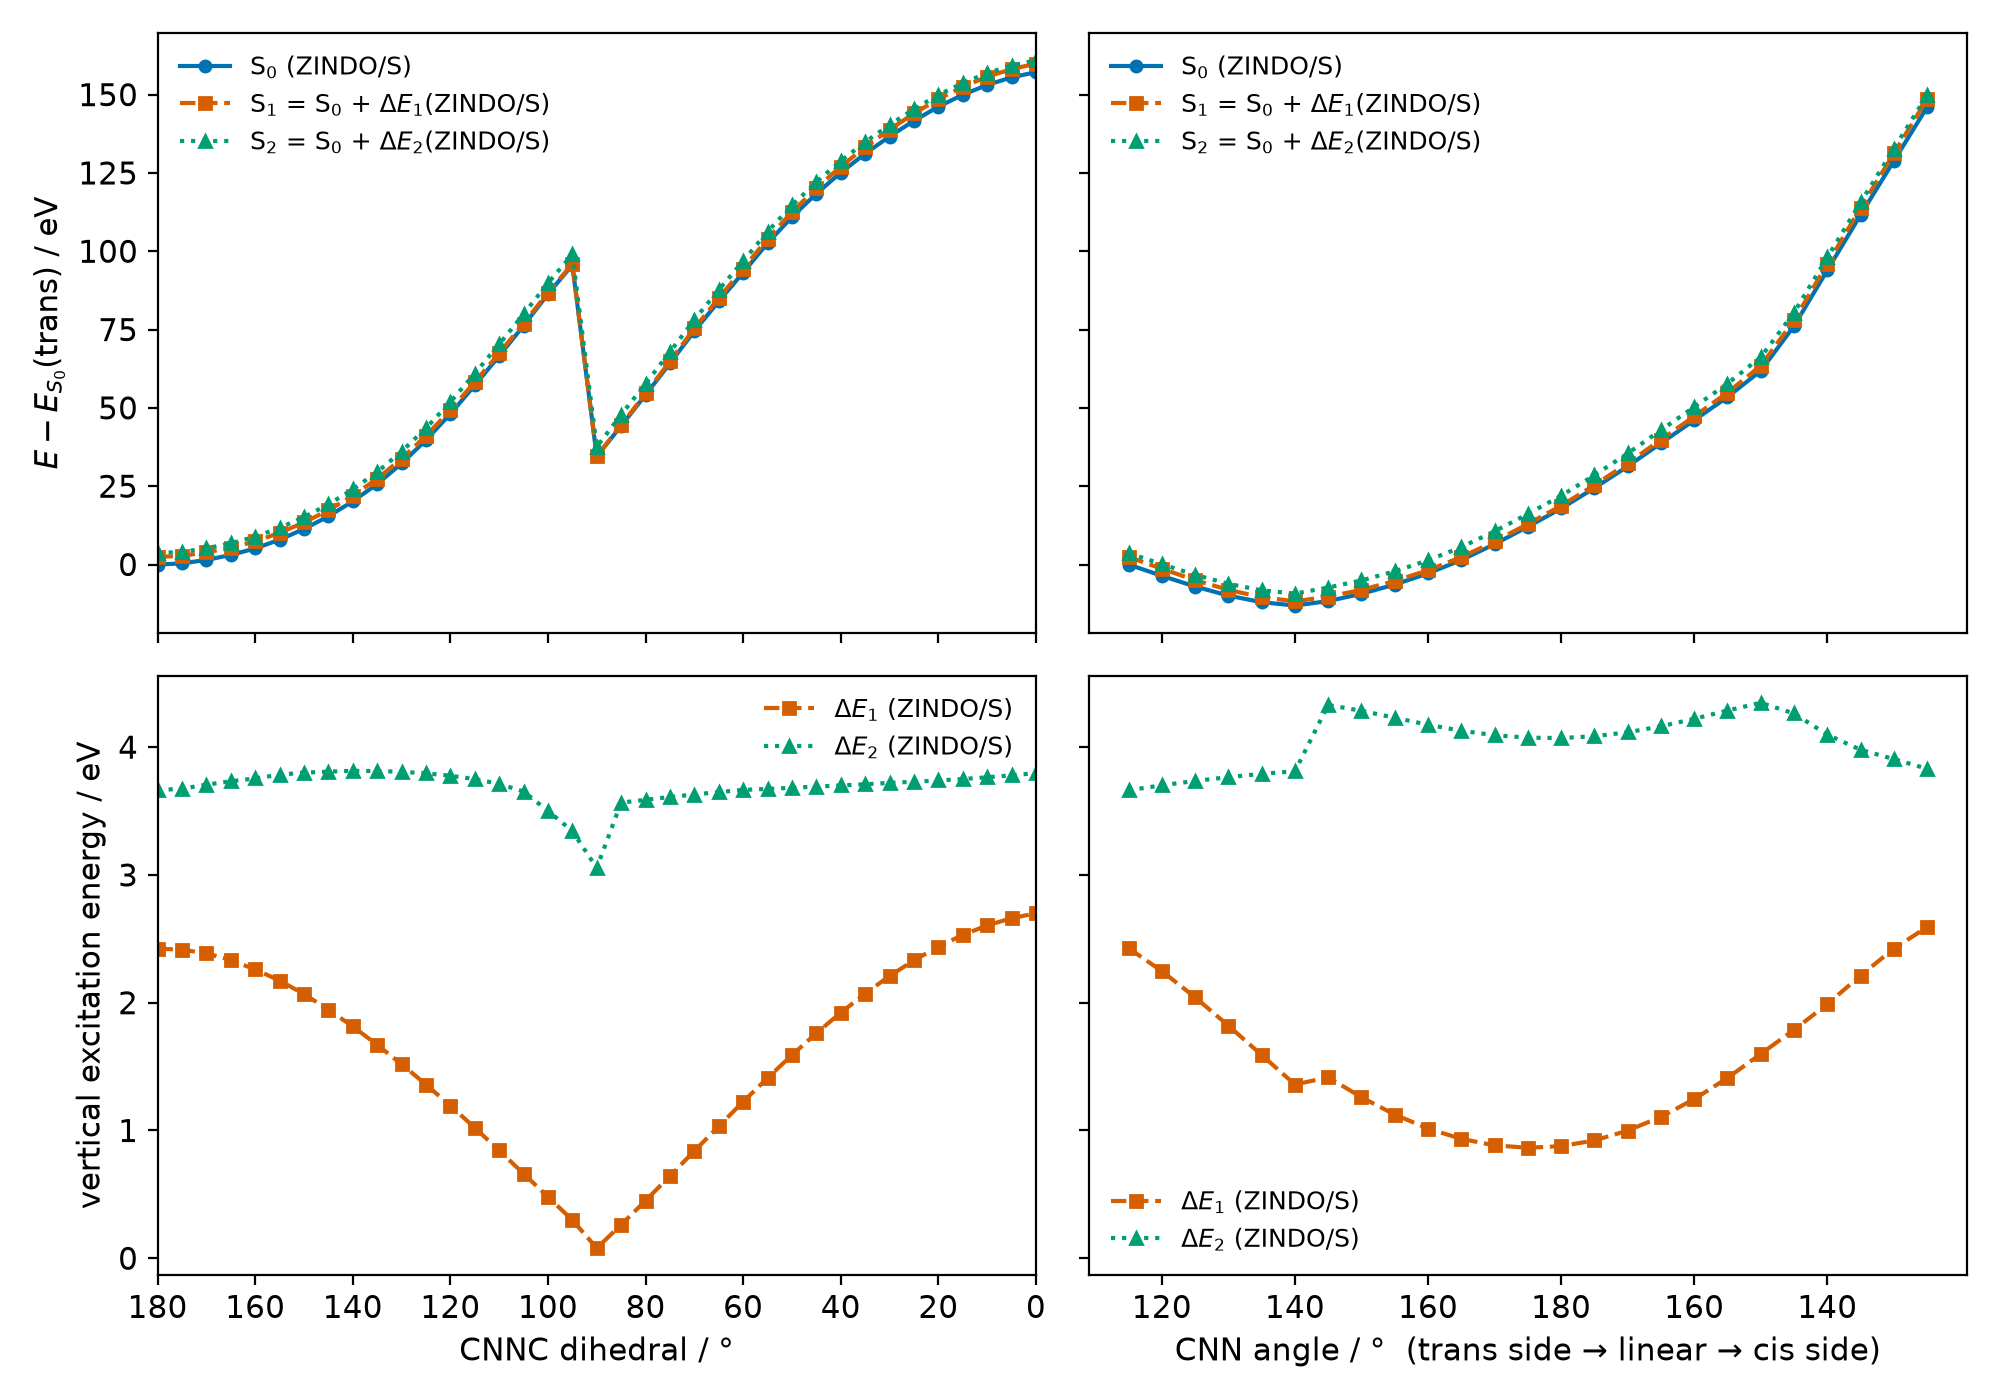
\includegraphics[width=\linewidth]{zindo_states.png}
\caption{Nahoře: $S_0$ (ZINDO/S, geometrie dolní obálky skenu) a~$S_n = S_0 + \Delta E_n$.
  Dole: vertikální excitační energie $\Delta E_n$ (ZINDO/S). Vlevo torze, vpravo inverze.}
\label{fig:zindo}
\end{figure}

Při torzi se $S_1$ k~\SI{90}{\degree} přibližuje k~$S_0$ až na $\Delta E_1 = \SI{0.08}{\electronvolt}$,
zatímco podél inverze zůstává $\Delta E_1 \geq \SI{0.86}{\electronvolt}$. Torzní cesta tedy vede
k~oblasti, kde se $S_1$ a~$S_0$ téměř dotýkají a~molekula se může z~$S_1$ nezářivě vrátit do
základního stavu. To odpovídá závěru, že stav $S_1$ se rozpadá hlavně po torzní cestě přes kónické
průniky u~CNNC \SIrange{95}{90}{\degree}~\cite{Cembran2004}. U~\SI{90}{\degree} je ale i~referenční
stav ZINDO/S uzavřenoslupkový, hodnota $\Delta E_1$ je proto jen kvalitativní. Skoky $\Delta E_2$ u~torze
\SI{90}{\degree} a~u~inverze mezi \SIlist{140;145}{\degree} odpovídají přechodu obálky mezi větvemi skenu,
nejsou to vlastnosti stavů.

\subsection*{Molekulové orbitaly a~charakter přechodů}
Orbital 29 má \SI{81}{\percent} hustoty na dusících a~leží v~rovině CNNC; odpovídá nevazebným
elektronovým párům dusíku (n). HOMO (33) a~LUMO (34) jsou orbitaly $\pi$ a~$\pi^*$ kolmé na rovinu
molekuly (obrázek~\ref{fig:mo}). Stav $S_1$ je v~obou izomerech přechod n$\to\pi^*$ (hlavně 29$\to$34)
a~$S_2$ přechod $\pi\to\pi^*$ (33$\to$34), viz tabulka~\ref{tab:exc}.

\begin{figure}[H]
\centering
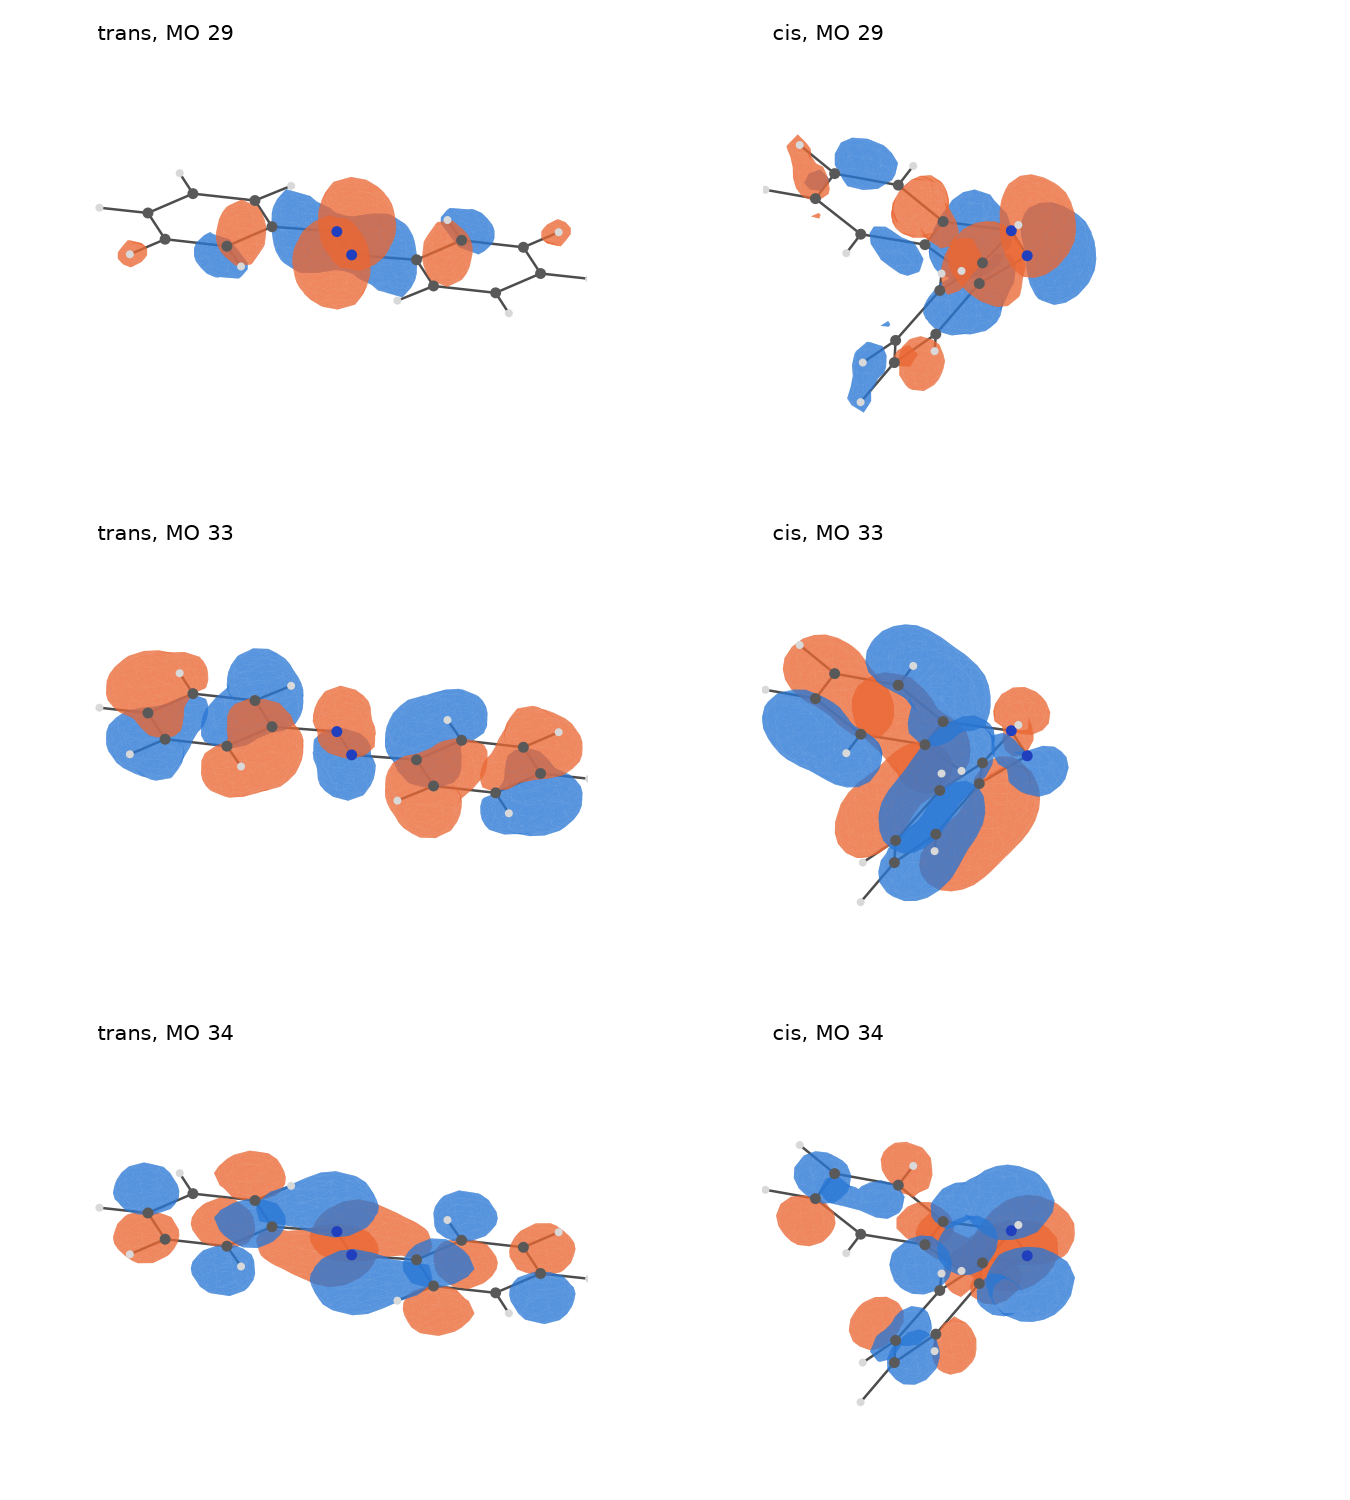
\includegraphics[width=0.75\linewidth]{orbitals.png}
\caption{Orbitaly ZINDO/S 29 (n), 33 (HOMO, $\pi$) a~34 (LUMO, $\pi^*$) pro \trans\ (vlevo) a~\cis\ (vpravo),
  izoplocha $\pm 0{,}03$.}
\label{fig:mo}
\end{figure}

\begin{table}[H]
\centering\small
\caption{Excitace ZINDO/S v~minimech: excitační energie $\Delta E$, síla oscilátoru $f$, hlavní excitace
  s~vahou v~závorce.}
\label{tab:exc}
\begin{tabular}{lSSlSSl}
\toprule
 & \multicolumn{3}{c}{\trans} & \multicolumn{3}{c}{\cis} \\
 & {$\Delta E$ / \si{\electronvolt}} & {$f$} & excitace & {$\Delta E$ / \si{\electronvolt}} & {$f$} & excitace \\
\midrule
$S_1$ & 2.42 & 0.000 & n$\to\pi^*$ (0,85) & 2.65 & 0.011 & n$\to\pi^*$ (0,69) \\
$S_2$ & 3.66 & 0.876 & $\pi\to\pi^*$ (0,96) & 3.78 & 0.177 & $\pi\to\pi^*$ (0,83) \\
\bottomrule
\end{tabular}
\end{table}

U~planárního \trans-izomeru je přechod n$\to\pi^*$ zakázaný ($f = 0$): orbital n leží v~rovině molekuly
a~$\pi^*$ je k~ní kolmý, takže přechodový dipólový moment je nulový ze symetrie. V~\cis-izomeru jsou
fenyly vytočené z~roviny CNNC, molekula není rovinná a~přechod už symetrií zakázán není; je slabě povolený
($f = 0{,}011$). Přechod $\pi\to\pi^*$ je intenzivní u~\trans\ ($f = 0{,}876$) a~u~\cis\ asi pětkrát slabší.
Ve spektru tedy očekáváme slabý pás n$\to\pi^*$ při nižší energii a~silný pás $\pi\to\pi^*$ při vyšší
energii; v~oblasti pásu n$\to\pi^*$ absorbuje více \cis-izomer.
\todo{případně doplnit srovnání s~experimentálními polohami pásů (se zdrojem)}

\section*{Závěr}
\begin{itemize}\itemsep2pt
  \item Oba izomery jsou minima (bez imaginárních frekvencí). \trans-azobenzen je stabilnější
        o~\SI{50.0}{\kilo\joule\per\mole} ($\Delta H$, $\omega$B97X-D3/def2-TZVP), experiment dává
        \SI{47}{\kilo\joule\per\mole}.
  \item \mbox{B3LYP/6-31G*} izomerační entalpii nadhodnocuje (\SI{61.9}{\kilo\joule\per\mole}),
        PM6 dává opačné znaménko (\SI{-16.5}{\kilo\joule\per\mole}).
  \item Tranzitní stav inverze leží \SI{116}{\kilo\joule\per\mole} nad \cis\
        ($E_\mathrm{a} = \SI{113}{\kilo\joule\per\mole}$, experiment \SI{118}{\kilo\joule\per\mole}).
        Torze kolem \SI{90}{\degree} vyžaduje výpočet s~otevřenými slupkami; triplet tam leží jen
        \SI{73}{\kilo\joule\per\mole} nad \cis.
  \item $S_1$ je přechod n$\to\pi^*$ (u~\trans\ zakázaný), $S_2$ intenzivní přechod $\pi\to\pi^*$. Podél
        torze se $S_1$ přibližuje k~$S_0$ na \SI{0.08}{\electronvolt}, podél inverze ne; ZINDO/S je
        použitelné jen pro excitační energie, ne pro energii základního stavu.
\end{itemize}

\begin{thebibliography}{99}\small\itemsep1pt
\bibitem{Jiang2026} Jiang, J.; Yuan, X.-R.; Hu, L. Recent Advances of Azobenzene-Based Photoresponsive
  Molecular Switches for Protein-Targeted Photopharmacology. \textit{Molecules} \textbf{2026}, 31, 1205
  (\href{https://doi.org/10.3390/molecules31071205}{DOI: 10.3390/molecules31071205}).
\bibitem{Gao2022} Gao, M.-H.; Kwaria, D.; Norikane, Y.; Yue, Y. Visible-Light-Switchable Azobenzenes:
  Molecular Design, Supramolecular Systems, and Applications. \textit{Nat. Sci.} \textbf{2022}, 3, e220020
  (\href{https://doi.org/10.1002/ntls.20220020}{DOI: 10.1002/ntls.20220020}).
\bibitem{Li2025} Li, S. Recent Advances in Visible Light-Triggered Azobenzene Photoswitches (A Review).
  \textit{Russ. J. Gen. Chem.} \textbf{2025}
  (\href{https://doi.org/10.1134/S1070363225605241}{DOI: 10.1134/S1070363225605241}).
  \todo{doplnit ročník a~strany}
\bibitem{Ryazantsev2021} Ryazantsev, M. N.; Strashkov, D. M.; Nikolaev, D. M.; Shtyrov, A. A.; Panov, M. S.
  Photopharmacological Compounds Based on Azobenzenes and Azoheteroarenes: Principles of Molecular Design,
  Molecular Modelling, and Synthesis. \textit{Russ. Chem. Rev.} \textbf{2021}, 90, 868–893
  (\href{https://doi.org/10.1070/RCR5001}{DOI: 10.1070/RCR5001}).
\bibitem{Cembran2004} Cembran, A.; Bernardi, F.; Garavelli, M.; Gagliardi, L.; Orlandi, G.
  On the Mechanism of the \textit{cis}–\textit{trans} Isomerization in the Lowest Electronic States of
  Azobenzene: S$_0$, S$_1$, and T$_1$. \textit{J. Am. Chem. Soc.} \textbf{2004}, 126, 3234–3243
  (\href{https://doi.org/10.1021/ja038327y}{DOI: 10.1021/ja038327y}).
\bibitem{Yamaguchi1988} Yamaguchi, K.; Jensen, F.; Dorigo, A.; Houk, K. N. A Spin Correction Procedure for
  Unrestricted Hartree-Fock and Møller-Plesset Wavefunctions for Singlet Diradicals and Polyradicals.
  \textit{Chem. Phys. Lett.} \textbf{1988}, 149, 537–542
  (\href{https://doi.org/10.1016/0009-2614(88)80378-6}{DOI: 10.1016/0009-2614(88)80378-6}).
\bibitem{Lin2013} Lin, Y.-S.; Li, G.-D.; Mao, S.-P.; Chai, J.-D. Long-Range Corrected Hybrid Density
  Functionals with Improved Dispersion Corrections. \textit{J. Chem. Theory Comput.} \textbf{2013}, 9, 263–272
  (\href{https://doi.org/10.1021/ct300715s}{DOI: 10.1021/ct300715s}).
\bibitem{Weigend2005} Weigend, F.; Ahlrichs, R. Balanced Basis Sets of Split Valence, Triple Zeta Valence and
  Quadruple Zeta Valence Quality for H to Rn. \textit{Phys. Chem. Chem. Phys.} \textbf{2005}, 7, 3297–3305
  (\href{https://doi.org/10.1039/b508541a}{DOI: 10.1039/b508541a}).
\bibitem{Neese2025} Neese, F. Software Update: The ORCA Program System, Version 6.0.
  \textit{WIREs Comput. Mol. Sci.} \textbf{2025}, 15, e70019
  (\href{https://doi.org/10.1002/wcms.70019}{DOI: 10.1002/wcms.70019}).
\bibitem{Becke1993} Becke, A. D. Density-Functional Thermochemistry. III. The Role of Exact Exchange.
  \textit{J. Chem. Phys.} \textbf{1993}, 98, 5648–5652
  (\href{https://doi.org/10.1063/1.464913}{DOI: 10.1063/1.464913}).
\bibitem{Lee1988} Lee, C.; Yang, W.; Parr, R. G. Development of the Colle-Salvetti Correlation-Energy Formula
  into a Functional of the Electron Density. \textit{Phys. Rev. B} \textbf{1988}, 37, 785–789
  (\href{https://doi.org/10.1103/PhysRevB.37.785}{DOI: 10.1103/PhysRevB.37.785}).
\bibitem{Stewart2007} Stewart, J. J. P. Optimization of Parameters for Semiempirical Methods V: Modification
  of NDDO Approximations and Application to 70 Elements. \textit{J. Mol. Model.} \textbf{2007}, 13, 1173–1213
  (\href{https://doi.org/10.1007/s00894-007-0233-4}{DOI: 10.1007/s00894-007-0233-4}).
\bibitem{MOPAC} MOPAC, verze 23.2.5. \url{https://github.com/openmopac/mopac}
  (staženo \todo{datum stažení}).
\bibitem{Ridley1973} Ridley, J.; Zerner, M. An Intermediate Neglect of Differential Overlap Technique for
  Spectroscopy: Pyrrole and the Azines. \textit{Theor. Chim. Acta} \textbf{1973}, 32, 111–134
  (\href{https://doi.org/10.1007/BF00528484}{DOI: 10.1007/BF00528484}).
\bibitem{Zhu2018} Zhu, M.; Yu, L. \textit{Trans}–\textit{cis} Isomerization Energies of Azopyridines:
  A Calorimetric and Computational Study. \textit{J. Therm. Anal. Calorim.} \textbf{2018}, 132, 463–469
  (\href{https://doi.org/10.1007/s10973-017-6913-0}{DOI: 10.1007/s10973-017-6913-0}).
\bibitem{Cammenga2009} Cammenga, H. K.; Emel'yanenko, V. N.; Verevkin, S. P. Re-investigation and Data
  Assessment of the Isomerization and 2,2'-Cyclization of Stilbenes and Azobenzenes.
  \textit{Ind. Eng. Chem. Res.} \textbf{2009}, 48, 10120–10128
  (\href{https://doi.org/10.1021/ie900800q}{DOI: 10.1021/ie900800q}).
\bibitem{Andersson1982} Andersson, J.-Å.; Petterson, R.; Tegnér, L. Flash Photolysis Experiments in the Vapour
  Phase at Elevated Temperatures I: Spectra of Azobenzene and the Kinetics of Its Thermal
  \textit{Cis}–\textit{Trans} Isomerization. \textit{J. Photochem.} \textbf{1982}, 20, 17–32
  (\href{https://doi.org/10.1016/0047-2670(82)80044-0}{DOI: 10.1016/0047-2670(82)80044-0}).
\end{thebibliography}

\end{document}
